% =====================================================================
%  CS5903 Final Project Report — Project 10, Group 37
%  Build:  pdflatex Project_Report.tex  (run twice for references)
%  Diagrams: Mermaid sources in diagrams/*.mmd, rendered to diagrams/*.pdf with
%            mmdc -i X.mmd -o X.pdf -f -c diagrams/cfg.json
%  Anything in \fillin{...} (red) is a value I still have to fill in.
% =====================================================================
\documentclass[11pt,a4paper]{article}

\usepackage[T1]{fontenc}
\usepackage[utf8]{inputenc}
\usepackage{lmodern}
\usepackage{microtype}
\usepackage[a4paper,margin=2.2cm,headheight=14pt]{geometry}
\usepackage{graphicx}
\usepackage{float}
\usepackage[table]{xcolor}
\usepackage{booktabs}
\usepackage{tabularx}
\usepackage{xltabular}
\usepackage{makecell}
\usepackage{enumitem}
\usepackage{caption}
\usepackage{fancyhdr}
\usepackage{titlesec}
\usepackage[most]{tcolorbox}
\usepackage{etoolbox}
\usepackage[hidelinks]{hyperref}
\AtBeginEnvironment{xltabular}{\small}

% ---------- look (follows the earlier progress report) ----------
\definecolor{accent}{HTML}{1F4E79}
\definecolor{okgreen}{HTML}{1B7F3B}
\definecolor{partial}{HTML}{B26A00}
\definecolor{notdone}{HTML}{A61B1B}
\definecolor{boxbg}{HTML}{F3F6FA}

\hypersetup{colorlinks=true,linkcolor=accent,urlcolor=accent,citecolor=accent}
\captionsetup{font=small,labelfont=bf}
\setlist{itemsep=2pt,topsep=3pt}
\renewcommand{\arraystretch}{1.18}
\setlength{\tabcolsep}{4.5pt}

\titleformat{\section}{\large\bfseries\color{accent}}{\thesection}{0.6em}{}
\titleformat{\subsection}{\normalsize\bfseries}{\thesubsection}{0.5em}{}
\titlespacing*{\section}{0pt}{12pt}{5pt}
\titlespacing*{\subsection}{0pt}{8pt}{3pt}

\pagestyle{fancy}
\fancyhf{}
\lhead{\small Final Project Report}
\rhead{\small Modular Learner Experience (P10-G37)}
\cfoot{\small\thepage}

\newcommand{\pass}{\textcolor{okgreen}{\textbf{Pass}}}
\newcommand{\passcode}{\textcolor{okgreen}{\textbf{Pass (code)}}}
\newcommand{\partl}{\textcolor{partial}{\textbf{Partial}}}
\newcommand{\notrun}{\textcolor{notdone}{\textbf{Not run}}}
\newcommand{\notdone}{\textcolor{notdone}{\textbf{Not done}}}
\newcommand{\fillin}[1]{\textcolor{red}{\textbf{[#1]}}}
\urlstyle{tt}
\makeatletter\g@addto@macro{\UrlBreaks}{\do\_\do\.\do\-\do\/}\makeatother
\newcommand{\fp}[1]{\nolinkurl{#1}}

\newcolumntype{L}[1]{>{\raggedright\arraybackslash}p{#1}}
\newcolumntype{Y}{>{\raggedright\arraybackslash}X}

\tcbset{notebox/.style={colback=boxbg,colframe=accent,boxrule=0.6pt,arc=2pt,left=6pt,right=6pt,top=4pt,bottom=4pt}}

\begin{document}
\sloppy
\raggedbottom

% =====================================================================
\begin{titlepage}
\centering
\vspace*{1.2cm}
{\Large\bfseries\color{accent} CS5903 — Final Project Report\par}
\vspace{0.6cm}
{\LARGE\bfseries Modular Mobile/Web Learner Experience with\\ Offline Synchronization and Agent-Driven UI\par}
\vspace{0.4cm}
{\large Project-1-DAT \;·\; Project 10 \;·\; Group 37\par}
\vspace{1.0cm}

\begin{tabularx}{0.95\textwidth}{@{}L{0.28\textwidth}Y@{}}
\toprule
Student & Shubham Yadav \quad (\fillin{roll no. — institute e-mail suggests CS26BTKMU11004}) \\
Group / project & Group 37 / Project 10 (single-member group) \\
Mobile + BFF repository & \url{https://github.com/shhubbhaam/agenticUI} (private) \\
Final tag & \texttt{cs5903-final-2026} (commit SHA given in the submission message) \\
Web modules repository & \url{https://github.com/shhubbhaam/learnhouse} (branch \texttt{dev}, \texttt{6a301103}) \\
LearnHouse deployment & \url{https://learn.praxisacademy.ai} \\
Report date & 21 November 2026 \\
\bottomrule
\end{tabularx}

\vspace{0.9cm}
\begin{tcolorbox}[notebox,width=0.92\textwidth,title={\bfseries Executive summary},colbacktitle=accent,coltitle=white]
\small
\textbf{Problem.} Learners need a mobile/web learning experience that keeps working through network
outages, lets an AI agent adapt the interface without ever executing agent-supplied code, and keeps
one source of truth for progress.\\[2pt]
\textbf{Delivered.} An Expo/React Native Android app and a thin Node backend-for-frontend (BFF) over a
self-hosted LearnHouse LMS. The BFF holds all secrets and sessions. The app has three switchable
feature modules (checkpoint player, assessment, agent UI); an agent-chosen Home layout rendered only
from a trusted, schema-validated catalogue; a SQLite outbox with a durable, idempotent BFF inbox; BFF
checkpoints with server grading; and an AI coach streamed over SSE with resume and a bound approval.
Three web feature modules (community image upload, Help \& Support tickets, weighted course grading)
were added to the team's LearnHouse fork.\\[2pt]
\textbf{Works today.} All 612 app tests (90 suites) and 121 BFF tests pass, and the app type-checks (21 Nov 2026).
Offline completion, sync and LearnHouse read-back were observed on the emulator. \textbf{Not done:}
measured M9 performance, recorded device evidence for M2/M4/M6/M8, a written preference-conflict rule
(S9), and independently deployable web modules (M3 was delivered inside LearnHouse by agreement).
\end{tcolorbox}
\end{titlepage}

\tableofcontents
\vspace{0.4cm}
\begin{tcolorbox}[notebox]
\small\textbf{How to read the status words.} \pass{} = an automated test or a recorded run shows it.
\passcode{} = automated tests pass but the matching device recording has not been made.
\partl{} = some of the outcome exists. \notrun{} / \notdone{} = no evidence. Fake-backed BFF tests run
against an in-memory LearnHouse double (\fp{bff/test/fakeLearnHouse.ts}); they prove BFF logic, not
LearnHouse's real routes. Nothing in this report is a measurement unless a unit and a source are given.
\end{tcolorbox}
\newpage

% =====================================================================
\section{Problem, scope and success criteria}

\subsection{Actors and problem statement}
\begin{itemize}
  \item \textbf{Learner} — uses the Android app (and the LearnHouse website) to follow one course.
  \item \textbf{Course staff} — author content, grade, and answer support tickets in LearnHouse.
  \item \textbf{AI agent (Gemini)} — proposes a Home layout and coaching suggestions; it is untrusted.
  \item \textbf{BFF operator} — runs the backend that holds the LearnHouse organisation token and the Gemini key.
\end{itemize}
The course problem statement (Project 10) asks for a cross-platform reference experience with
modular mobile architecture, independently deployable web modules, a shared contract, a
checkpoint-aware media player, offline event synchronization and protocol-based agent/UI interaction,
where agent UI renders only from a trusted catalogue and offline behaviour is tested with multi-device
conflicts. Only public or synthetic data may be used.

\subsection{Scope}
\begin{xltabular}{\textwidth}{L{0.47\textwidth}Y}
\toprule
\textbf{In scope (delivered or attempted)} & \textbf{Out of scope / not attempted} \\
\midrule
One native target (Android emulator) and one LearnHouse course; LearnHouse remains the LMS. &
A new LMS or course database; iOS device testing; runtime-loaded mobile modules. \\
Thin BFF for secrets, sessions, policy and the extension records LearnHouse lacks (event inbox, checkpoints, coach). &
Full AG-UI or A2UI protocol conformance (an AG-UI-\emph{style} subset is implemented). \\
Three mobile feature modules: player, assessment, agent UI. &
Agent streaming on the web client (M6 allows one client). \\
Three web feature modules inside the LearnHouse fork (approved change, §6.2). &
Module-Federation shell with separately deployed web remotes. \\
\bottomrule
\end{xltabular}

\subsection{Assumptions and constraints}
\begin{itemize}
  \item Single-member group; the W3 plan budgeted about 12\,h/week (\fp{docs/W3-plan-and-evidence.md} §4). Actual hours were not logged weekly.
  \item The LearnHouse instance is the team's self-hosted fork at \texttt{learn.praxisacademy.ai}. Its public \texttt{/openapi.json} is disabled, so the deployed commit is not pinned from the API (§8).
  \item Course content is the real cohort course allow-listed in \fp{bff/.env}; checkpoint questions are synthetic (\fp{bff/checkpoints.json}).
  \item Gemini free tier; the model may be unavailable (an HTTP 503 fallback was observed on 24 Oct 2026).
\end{itemize}

\subsection{Approved milestones and the ``done when'' workflow}
The nine milestones M1–M9 and 13 acceptance scenarios S1–S13 come from the project sheet and the Week 0
review. They were mapped to binary test groups (T1.1 … T9.2) with thresholds in the W3 plan dated
11 Oct 2026 — two days after the 9 Oct freeze deadline (recorded honestly in ADR-004).
\begin{tcolorbox}[notebox]
\small\textbf{Done when} (project sheet): a learner can use a modular mobile or web client to consume
learning content, complete checkpoint interactions, work through a network outage, resume synchronized
state and interact with an agent that streams state and safely renders approved dynamic UI, with
accessibility and failure tests passing.\\[3pt]
\textbf{Target metrics frozen in the W3 plan:} cold start $\le$ 3\,s (median of 5, emulator); web bundle
$\le$ 500\,KB gzip; reconnect-to-synced $\le$ 5\,s after a 60\,s outage; resume drift $\le$ 1\,s; 0
skipped/duplicated checkpoints; 200\% font scale with no clipped call-to-action; contrast $\ge$ 4.5:1.
\end{tcolorbox}

% =====================================================================
\section{Related work, baselines and alternatives}

\subsection{Prior systems and reused tools}
Learner models are a central concern in adaptive e-learning \cite{wang2025}. Google's A2UI describes
agent-proposed interfaces as declarative, catalogue-bound components rendered by the client
\cite{a2ui}; AG-UI defines lifecycle, text, tool-call, state and interrupt events for agent–UI
streams \cite{agui}. This project applies both ideas in a reduced, documented subset rather than
adopting either SDK.

\begin{xltabular}{\textwidth}{L{0.22\textwidth}L{0.17\textwidth}L{0.12\textwidth}Y}
\toprule
\textbf{Reused} & \textbf{Version} & \textbf{Licence} & \textbf{What the project added} \\
\midrule
LearnHouse LMS \cite{learnhouse} & fork of v1.3.7 & AGPL-3.0 & Three web feature modules (§3.6); used unchanged as the LMS behind the BFF. \\
Expo / React Native & SDK 58 / RN 0.88.0 & MIT & All app screens, modules, local storage and sync. \\
expo-sqlite, expo-video & 58.0.x & MIT & Outbox, saved trail, playhead; hosted-video playback. \\
react-native-youtube-iframe & 2.4.x & MIT & YouTube lesson playback (supervisor's direction). \\
Zod & 4.x & MIT & All shared contracts (layout, events, checkpoints, agent events). \\
Node.js \texttt{node:http}, \texttt{node:sqlite} & Node $\ge$ 22.11 & MIT & Dependency-free BFF and its inbox. \\
Gemini API \cite{gemini} & \fp{gemini-3.5-flash-lite} & Google terms & Structured-output calls only, behind the BFF. \\
\bottomrule
\end{xltabular}

\subsection{Approaches considered}
\begin{xltabular}{\textwidth}{L{0.2\textwidth}L{0.33\textwidth}Y}
\toprule
\textbf{Approach} & \textbf{For} & \textbf{Against} \\
\midrule
Rule-based layout only & Deterministic, cheap, testable. & Rules multiply with signals; no adaptive coaching. \\
Agent-generated UI code & Maximum flexibility. & Executes untrusted code; impossible to validate; rejected by the project constraints. \\
\textbf{Hybrid: agent selects from a trusted catalogue (chosen)} & Agent adapts content and composition; the app owns components, actions and styles; output is validated on both sides. & Quality depends on the model; a valid layout is not necessarily a good one. \\
\bottomrule
\end{xltabular}
\textbf{Working baseline.} The rule-based alternative is kept in the code: when Gemini is absent,
fails or times out, the BFF serves a deterministic layout built from LearnHouse data
(\fp{bff/src/agent.ts}, \texttt{fallbackSlots}); the coach falls back to fixed template wording.
No systematic comparison of the two was run (§5).

% =====================================================================
\section{Architecture and implementation}

\begin{figure}[H]
\centering
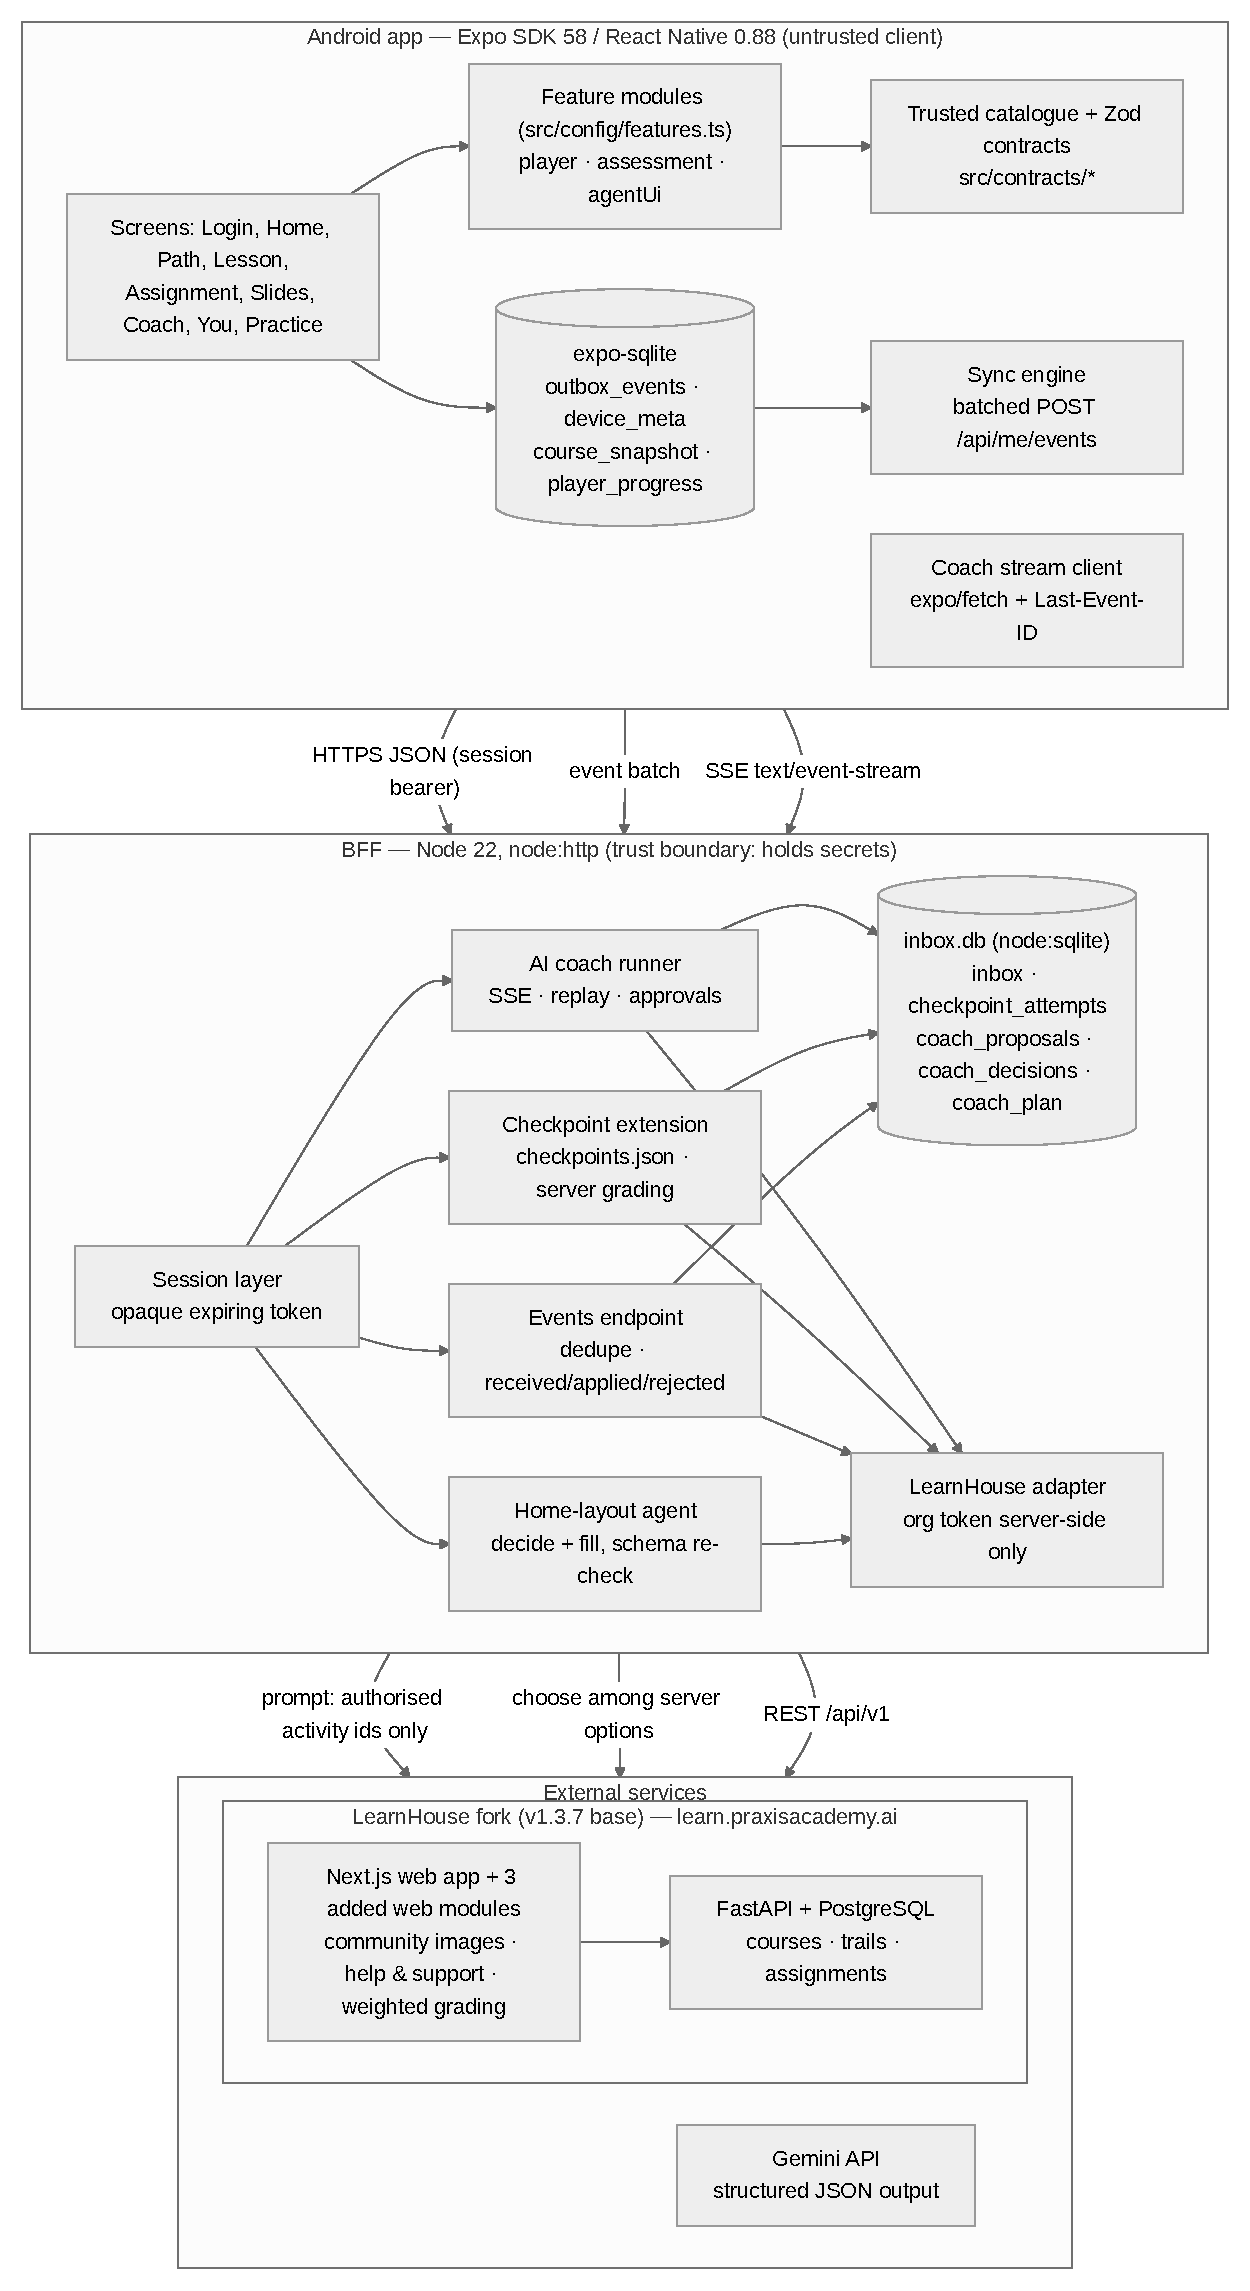
\includegraphics[width=0.78\textwidth]{diagrams/system-architecture.pdf}
\caption{Components, data flow and trust boundaries. Source: \fp{diagrams/system-architecture.mmd}.}
\label{fig:arch}
\end{figure}

\subsection{Components and interfaces}
\begin{xltabular}{\textwidth}{L{0.21\textwidth}L{0.29\textwidth}Y}
\toprule
\textbf{Component} & \textbf{Source} & \textbf{Responsibility / interface} \\
\midrule
Shared contracts & \fp{src/contracts/} & Zod schemas imported by app and BFF: home layout, events, checkpoints, assignment, agent events. \\
Feature switches & \fp{src/config/features.ts}, \fp{src/navigation/activityRoute.ts} & Turn \texttt{player}, \texttt{assessment}, \texttt{agentUi} off independently; a disabled module's routes open a ``turned off'' screen. \\
Local storage & \fp{src/data/local/} & SQLite tables \texttt{outbox\_events}, \texttt{device\_meta}, \texttt{course\_snapshot}, \texttt{player\_progress}, settings. \\
Sync engine & \fp{src/data/sync/syncEngine.ts} & Sends the outbox in batches (max 100) to \texttt{POST /api/me/events}; applies per-event results. \\
BFF sessions & \fp{bff/src/sessions.ts}, \fp{bff/src/app.ts} & LearnHouse login → opaque expiring session; every \texttt{/api/me/*} route derives learner from it. \\
LearnHouse adapter & \fp{bff/src/learnhouse.ts} & Only place that holds the org token; trail, meta, completion, assignment calls. \\
Home-layout agent & \fp{bff/src/agent.ts} & Two Gemini stages (choose components, fill props), then the app's own \texttt{parseHomeLayout} and target checks. \\
Event inbox & \fp{bff/src/inbox.ts} & Durable dedupe by event id + payload hash; \texttt{received} vs \texttt{applied}. \\
Checkpoints & \fp{bff/src/checkpointStore.ts}, \fp{bff/checkpoints.json} & Questions without answers to the app; grading and append-only attempts on the server. \\
AI coach & \fp{bff/src/coach*.ts}, \fp{src/screens/coach/} & SSE session with replay, snapshot and bound approval (§3.5). \\
\bottomrule
\end{xltabular}

\textbf{BFF HTTP API.} \texttt{POST /api/auth/login|logout}; \texttt{GET /api/me}, \texttt{/api/me/trail};
\texttt{GET /api/me/courses/:c/meta|trail|home-layout}; \texttt{POST …/activities/:a/complete};
\texttt{POST /api/me/events}; \texttt{GET …/activities/:a/checkpoints}, \texttt{POST …/checkpoints/:id/answer};
\texttt{…/video}, \texttt{…/slides}, \texttt{…/assignment}; \texttt{POST /api/me/coach/sessions},
\texttt{GET …/sessions/:id/events} (SSE), \texttt{POST …/cancel}, \texttt{POST /api/me/coach/approvals/:id},
\texttt{GET /api/me/coach/status}.

\subsection{State ownership and security boundary}
\begin{xltabular}{\textwidth}{L{0.36\textwidth}L{0.2\textwidth}Y}
\toprule
\textbf{State} & \textbf{Owner} & \textbf{Notes} \\
\midrule
Courses, activities, enrolment, completion, quiz submissions, grades & LearnHouse & BFF writes, then always reads back. \\
Event inbox, checkpoint attempts, coach proposals/decisions/plan & BFF (\fp{bff/data/inbox.db}) & Extension records keyed by LearnHouse ids. \\
Pending events, saved trail, device id and sequence, playhead & App (SQLite) & Pending rows deleted once \texttt{applied}. \\
Sessions, coach event log & BFF memory & Lost on BFF restart: the learner signs in again; open proposals are void. \\
\bottomrule
\end{xltabular}
Secrets (\texttt{LH\_API\_TOKEN}, \texttt{GEMINI\_API\_KEY}) exist only in \fp{bff/.env} (git-ignored;
\fp{bff/.env.example} has placeholders). The model receives activity titles, ids and counts — no name,
e-mail or raw answers — and model text is never logged (ADR-002, ADR-013).

\subsection{Declarative generated UI (M7)}
\begin{figure}[H]
\centering
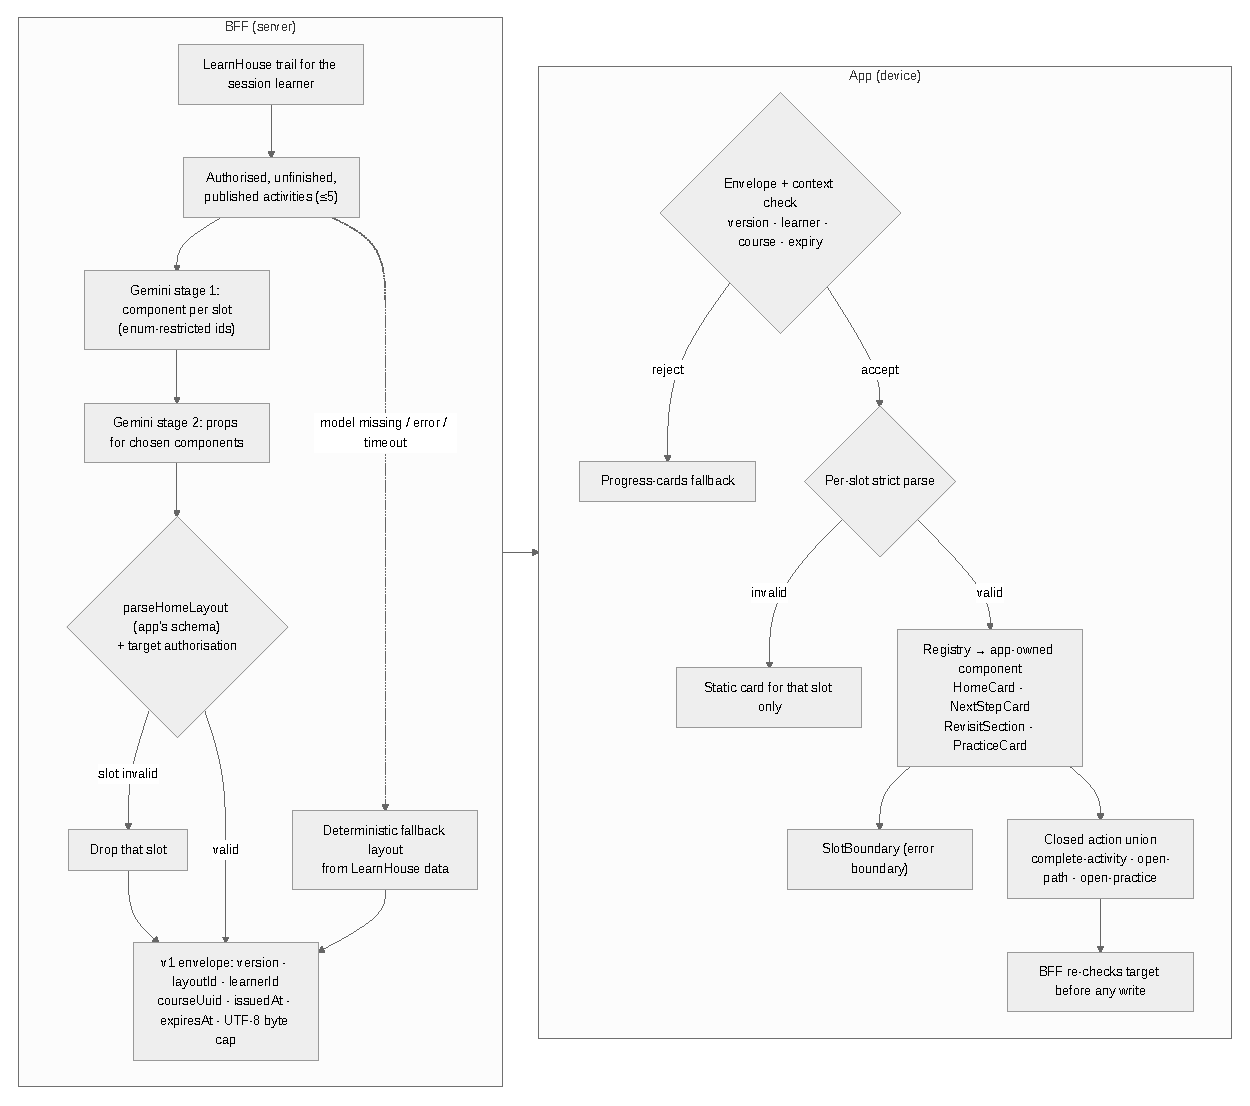
\includegraphics[width=0.92\textwidth]{diagrams/declarative-ui-pipeline.pdf}
\caption{Agent-chosen Home layout: validated by the BFF with the app's schema, then again per slot on the device.}
\end{figure}
The catalogue holds four components (\texttt{HomeCard}, \texttt{NextStepCard}, \texttt{PracticeCard},
\texttt{RevisitSection}) and three actions (\texttt{complete-activity}, \texttt{open-path},
\texttt{open-practice}). Envelopes carry version, layout id, learner, course, issue and expiry times
and are capped in UTF-8 bytes. A slot that fails parsing or throws while rendering falls back alone
(\fp{src/ui/organisms/SlotBoundary.tsx}).

\subsection{Offline-first synchronization (M5)}
\begin{figure}[H]
\centering
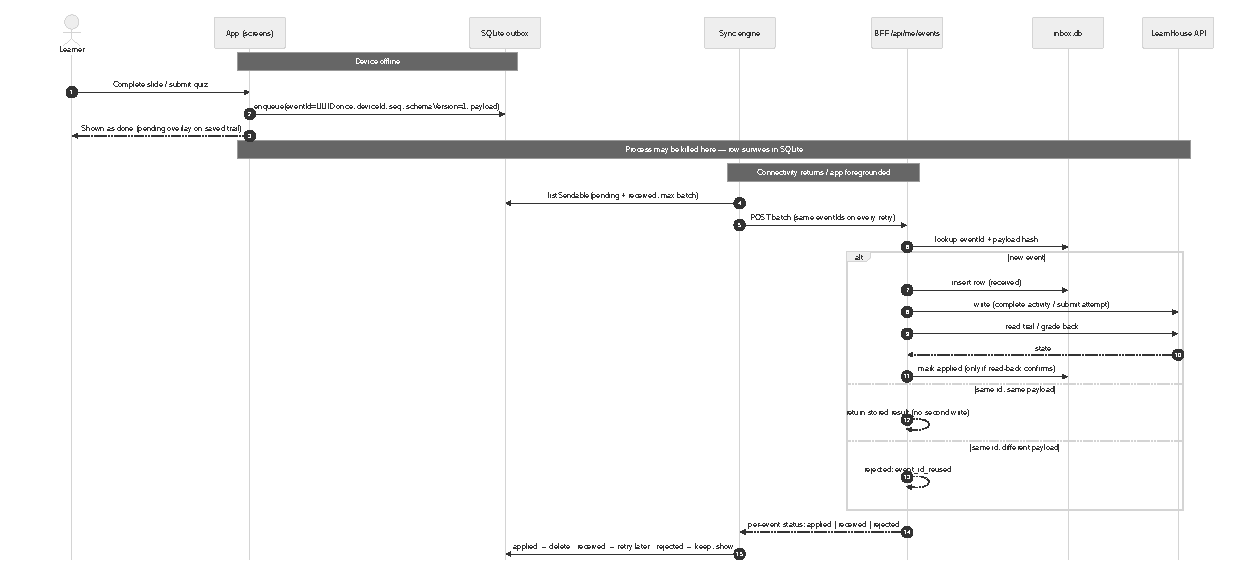
\includegraphics[width=0.95\textwidth]{diagrams/offline-sync-sequence.pdf}
\caption{Offline completion, durable outbox, idempotent upload and read-back.}
\end{figure}
Conflict rules by data type: completion is monotonic (never undone); quiz hand-ins are append-only
attempts with stage markers (\texttt{retried} → \texttt{submitting}) so a resend never submits twice,
and a lost response is resolved by reading the grade back; events with an unsupported
\texttt{schemaVersion} or a reused id with a different payload are rejected and kept visible on the
device. Offline, the app shows the last saved trail with pending completions overlaid.

\subsection{Checkpoint player (M4) and agent protocol (M6)}
\begin{figure}[H]
\centering
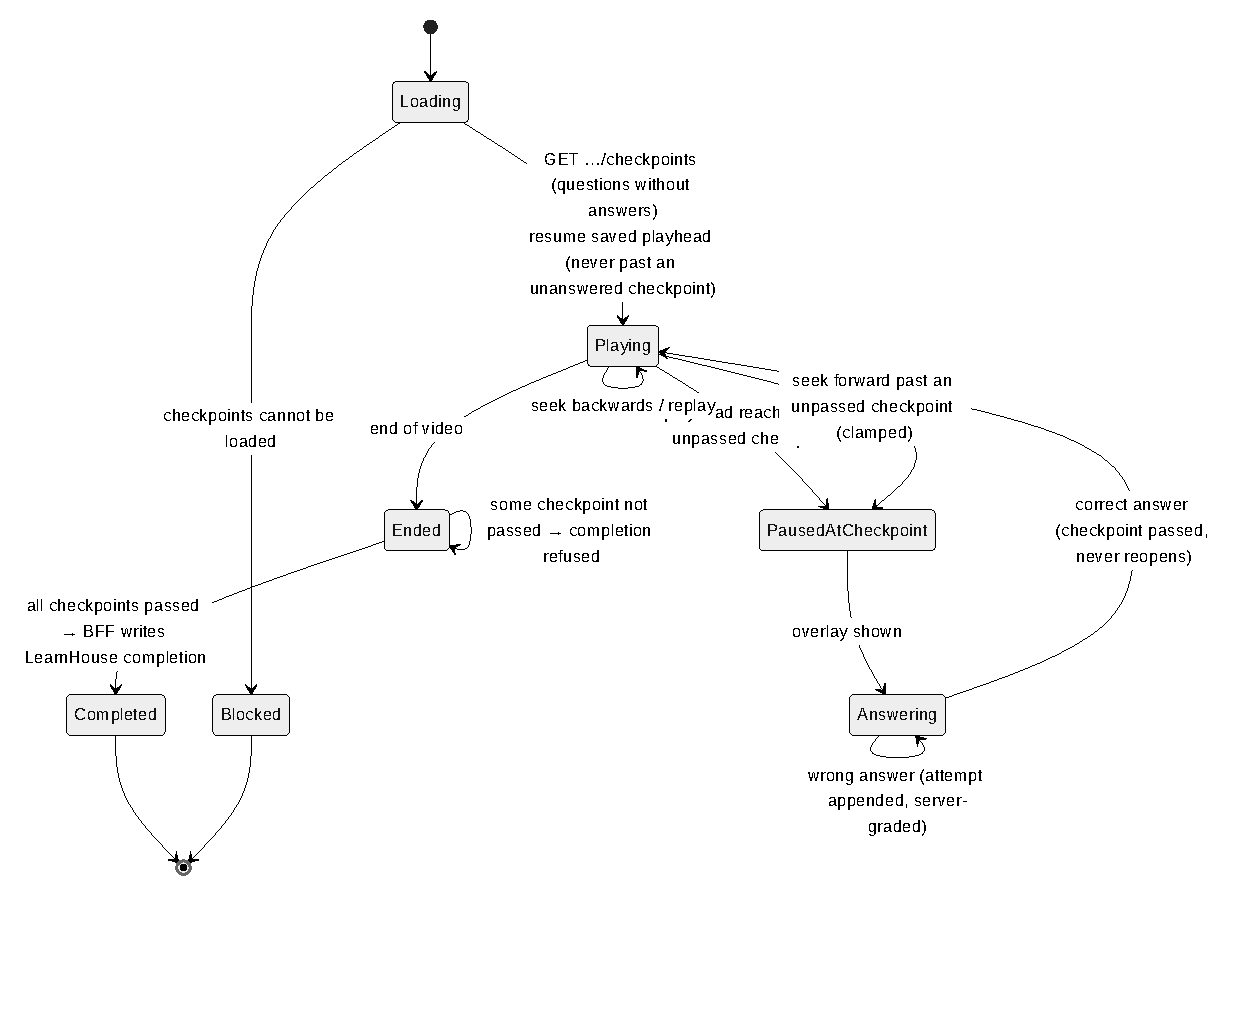
\includegraphics[width=0.72\textwidth]{diagrams/checkpoint-player-flow.pdf}
\caption{Checkpoint player states (M4).}
\end{figure}
\begin{figure}[H]
\centering
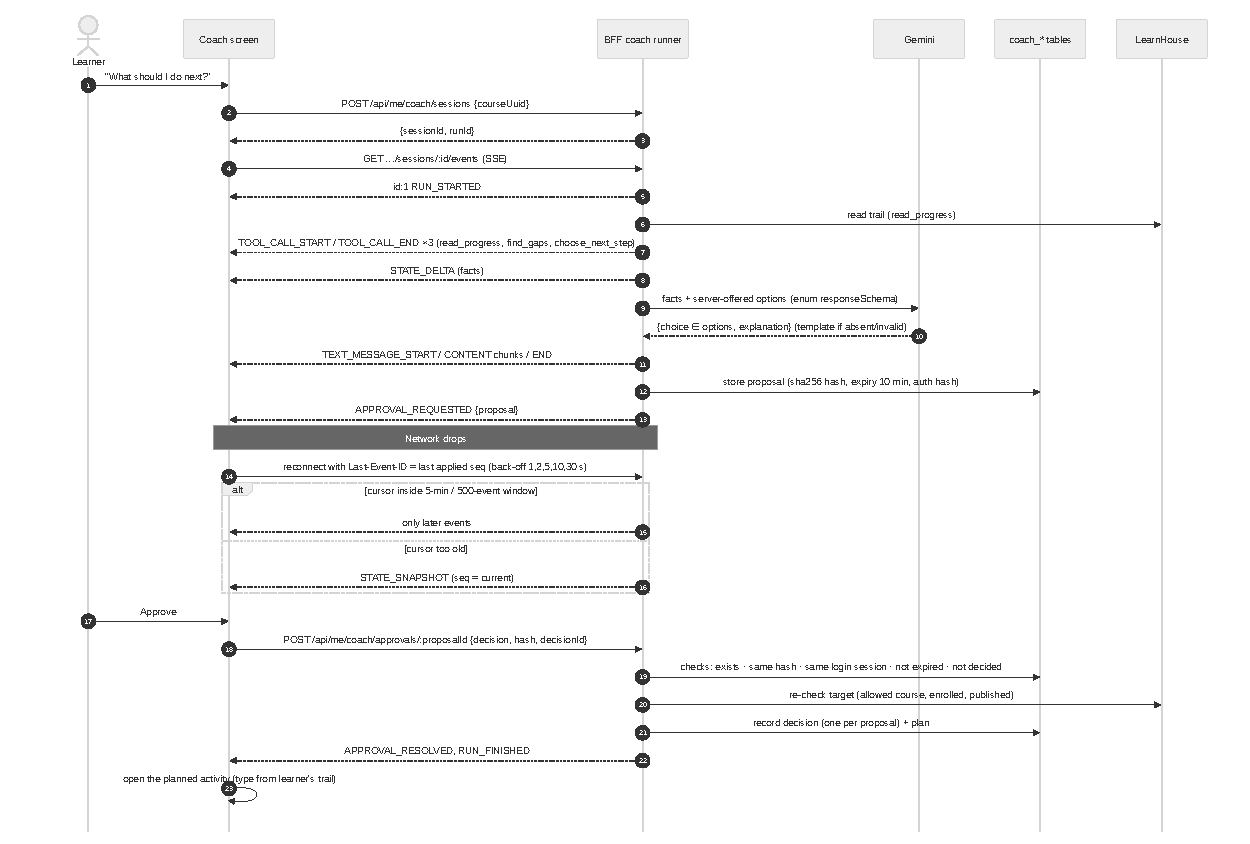
\includegraphics[width=\textwidth]{diagrams/coach-sse-sequence.pdf}
\caption{AI coach session over SSE with resume and a bound approval (M6).}
\end{figure}
\textbf{M4.} LearnHouse has no checkpoints, so they are a BFF extension. The player pauses exactly at
each unpassed checkpoint, cannot seek past one, never reopens a passed one, and resumes the saved
playhead; LearnHouse completion is refused until all checkpoints are passed.\\
\textbf{M6.} Event envelope \{schemaVersion, seq, sessionId, runId, at, type, payload\} with types
\texttt{RUN\_STARTED}, \texttt{TOOL\_CALL\_START/END}, \texttt{STATE\_SNAPSHOT/DELTA},
\texttt{TEXT\_MESSAGE\_START/CONTENT/END}, \texttt{APPROVAL\_REQUESTED/RESOLVED},
\texttt{RUN\_FINISHED}, \texttt{RUN\_ERROR}. Replay window 5\,min / 500 events, heartbeat every 15\,s,
client back-off 1, 2, 5, 10, 30\,s and a 45\,s stall watchdog. A proposal carries a SHA-256 hash and
10-minute expiry; one decision per proposal; it is bound to the learner and login session and the
target is re-checked when the decision runs. The coach is isolated from the Home layout (own
contract, routes, model call, tables). After approval the app opens the planned activity.

\subsection{Web modules in the LearnHouse fork (M3, approved change)}
By agreement with the reviewer, the web part of the project was built as three feature modules inside
the team's LearnHouse fork (\url{https://github.com/shhubbhaam/learnhouse}, branch \texttt{dev}, based on
upstream release 1.3.7) rather than as a separate web shell (ADR-009). Each module adds back-end code to
the LearnHouse API (FastAPI, SQLModel, Alembic migrations) and front-end code to the LearnHouse web app
(Next.js), and reuses LearnHouse's sign-in, organisation roles (RBAC), page routing, design components
and translation files. I wrote all three.

\begin{figure}[H]
\centering
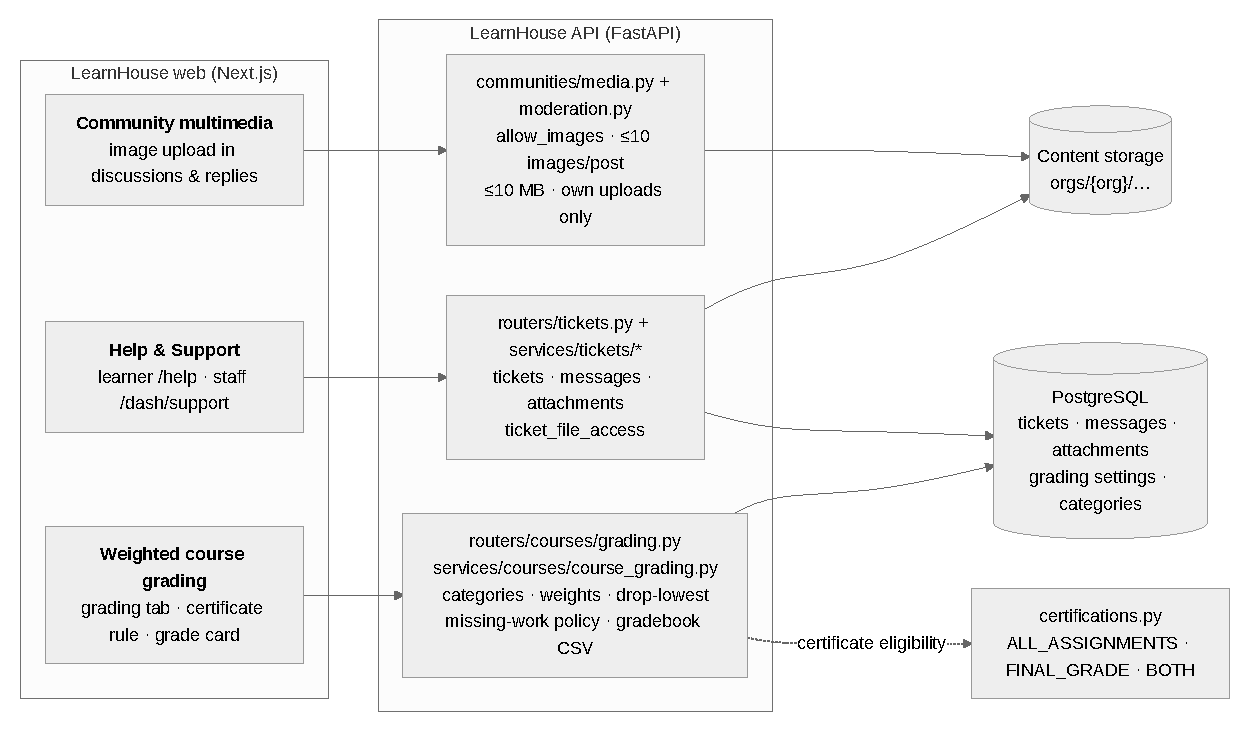
\includegraphics[width=\textwidth]{diagrams/web-modules.pdf}
\caption{The three web feature modules: web pages, API code and storage. Source: \fp{diagrams/web-modules.mmd}.}
\end{figure}

\begin{xltabular}{\textwidth}{L{0.2\textwidth}L{0.22\textwidth}L{0.2\textwidth}Y}
\caption{Summary of the web modules.}\label{tab:web}\\
\toprule
\textbf{Module} & \textbf{Commits (date)} & \textbf{Size} & \textbf{Tests written} \\
\midrule
Community multimedia upload & \texttt{4adc2055} (12 Oct 2026) & 25 files & 24 API \\
Help \& Support & \texttt{d39e16c7} (30 Oct), \texttt{1108064b} (21 Nov 2026) & 17 + 57 files & 68 API, 19 web \\
Weighted course grading & \texttt{04829b8f}, \texttt{6a301103} (21 Nov 2026) & 9 + 19 files & 39 API, 18 web \\
\bottomrule
\end{xltabular}

% ---------------------------------------------------------------
\subsubsection*{3.6.1 Community multimedia upload}
\textbf{Problem.} LearnHouse community discussions accepted only text, so learners could not share a
screenshot of an error or a diagram when asking for help.

\textbf{What the user sees.} In the discussion editor and the reply box, an image button (and
pasting or dropping an image) uploads the picture and inserts it into the post. Posts and replies
show their images in a grid (\fp{CommentImages.tsx}). In the community's moderation settings, staff
can switch images off for that community (\texttt{allow\_images}, on by default).

\textbf{How it works.}
\begin{enumerate}
  \item The browser uploads each image to \texttt{POST /communities/\{community\_uuid\}/media}
        (\fp{apps/api/src/services/communities/media.py}). Anyone who can read the community may upload,
        unless images are switched off. The server stores the file under the organisation's content
        folder and returns its file id.
  \item The post is saved as rich content in which each image is a \texttt{communityImage} node that
        refers to that file id.
  \item When the post or reply is saved, \fp{moderation.py} walks the whole content tree and rejects it
        if any rule fails, with a fixed error code.
\end{enumerate}

\textbf{Rules the server enforces.} Images allowed only when the community setting is on; only files
uploaded to \emph{this} community are accepted, so a post cannot hot-link outside images (which could
track readers); at most 10 images per post; 10\,MB per image (below LearnHouse's general 15\,MB image
limit); alt text at most 300 characters; text formatting limited to bold, italic, strike, code, link
and underline; links limited to \texttt{http}, \texttt{https} and \texttt{mailto}. The web client offers
JPEG, PNG, GIF and WebP files.

\textbf{Tests.} 24 tests in \fp{apps/api/src/tests/services/test_community_rich_content.py}
(not run for this report, §5.1).

% ---------------------------------------------------------------
\subsubsection*{3.6.2 Help \& Support}
\textbf{Problem.} LearnHouse had no way for a learner to ask the course team for help inside the
platform, or for staff to track those requests.

\textbf{Learner side} (\texttt{/orgs/\{org\}/help}, linked from the organisation menu). The learner raises a ticket with a subject (up to 200 characters), a description (up to 10\,000),
a category (technical, course content, billing, account, other), a priority (low, medium, high,
urgent) and optionally the course it is about. They see a list of their own tickets with status
badges, open one to read the conversation, reply, and attach screenshots. Replying to a resolved ticket
reopens it; a closed ticket cannot be replied to.

\textbf{Staff side} (\texttt{/dash/support} in the dashboard). Organisation admins and maintainers get a
support queue they can filter by status, priority, category and ``assigned to me'', open a ticket, change its status
(open, in progress, resolved, closed) and priority, assign it to another admin or maintainer, write a
resolution note when resolving, close it, and add \emph{internal notes} that the learner never sees.

\begin{xltabular}{\textwidth}{L{0.42\textwidth}Y}
\toprule
\textbf{API route} (\fp{apps/api/src/routers/tickets.py}) & \textbf{Who / what} \\
\midrule
\texttt{POST /tickets/} & Any member of the organisation: raise a ticket \\
\texttt{GET /tickets/org/\{org\_id\}/me} & The learner's own tickets \\
\texttt{GET /tickets/org/\{org\_id\}/admin} & Staff only: the support queue with filters \\
\texttt{GET /tickets/\{ticket\_uuid\}} & Owner or staff: the ticket and its thread \\
\texttt{PATCH /tickets/\{ticket\_uuid\}} & Staff only: status, priority, assignee, resolution note \\
\texttt{POST /tickets/\{ticket\_uuid\}/messages} & Owner or staff: reply (staff may mark it internal) \\
\texttt{POST /tickets/\{ticket\_uuid\}/attachments} & Owner or staff: upload an image before sending \\
\bottomrule
\end{xltabular}

\textbf{Data.} Three new tables, created by Alembic migrations \texttt{e1ebd9e62249} and
\texttt{f2a3b4c5d6e7}: \texttt{SupportTicket} (subject, description, category, priority, status,
resolution note, organisation, learner, optional course, assignee, dates), \texttt{TicketMessage}
(author, text, \texttt{is\_staff}, \texttt{is\_internal}) and \texttt{TicketAttachment} (file, type,
size, uploader, whether it is internal, which message it belongs to).

\textbf{Access rules.} Only signed-in organisation members can use tickets; API tokens are refused. A
learner who is not the owner gets ``not found'' rather than ``forbidden'', so ticket ids cannot be
probed. Only staff can triage, assign, or write internal notes, and tickets can be assigned only to
admins or maintainers of the same organisation.

\textbf{Attachments.} The browser uploads each image first; the server stores it and records a
\emph{pending} row. Sending the reply links those rows to the message; every id must be a pending
upload by the same user on the same ticket. Limits: JPEG, PNG, GIF or WebP; 10\,MB each; 5 per message;
20 pending uploads per user. LearnHouse normally serves everything under \texttt{orgs/} publicly, which
would let anyone with a link see a learner's screenshot. A new check
(\fp{apps/api/src/security/ticket_file_access.py}) runs first in both content routes and allows a ticket
file only if an attachment row exists for exactly that ticket and file, and the caller is staff, the
uploader, or the ticket owner (owners never see internal-note images).

\textbf{Also delivered.} English and Arabic interface strings; two Postman collections for the API;
the design and plan documents for the front end.

\textbf{Tests.} API: 4 router, 48 service and 16 file-access tests. Web: 8 attachment, 8 filter and 3
request tests (\fp{apps/web/tests/}). Not run for this report (§5.1).

% ---------------------------------------------------------------
\subsubsection*{3.6.3 Weighted course grading}
\textbf{Problem.} LearnHouse graded each assignment separately and issued a certificate only when
every graded assignment was passed. A course could not say, for example, ``quizzes are 30\% and the
project is 70\%'', drop a learner's worst quiz, or certify on a final grade.

\textbf{Staff side.} A new \emph{Grading} tab in the course editor (\fp{EditCourseGrading.tsx}) sets:
the grading mode (``all must pass'', the old behaviour and the default, or ``weighted''); categories
with names and weights; ``drop the lowest $k$'' per category; each assignment's category, its weight
inside the category and a \emph{never drop} flag (also editable from the assignment dialog); what
happens to missing work (counts as 0\% after the due date, or is left out); the final grade format
(percentage, numeric, letter, GPA scale or pass/fail, reusing LearnHouse's assignment grade formats) and pass mark;
and the certificate rule. Staff can open a gradebook for the whole course and export it as CSV.

\textbf{Learner side.} The course page shows a grade card (\fp{CourseGradeCard.tsx}) with the current
course grade and the score of each category.

\textbf{How the grade is calculated} (\fp{apps/api/src/services/courses/course_grading.py}):
\begin{enumerate}
  \item Each assignment is classified for the learner: \emph{graded} (its percentage), \emph{missing}
        (not handed in, past due, and the course counts missing work as 0\%), \emph{pending} (not yet
        counted) or left out (formative, or nothing to grade).
  \item Each category averages its assignments, weighted by each assignment's weight. Its lowest
        $k$ scores are dropped, but only once the learner has no pending item in that category, and
        never an assignment marked \emph{never drop}.
  \item The course percentage is the weighted average of the category percentages, divided only by
        the weights of categories that already have a score, so a learner half-way through sees a fair
        current grade.
  \item The percentage is shown in the course's grade format and compared with its pass mark.
\end{enumerate}
The calculation is in pure functions with no database access, so it is unit-tested directly.

\textbf{Validation when staff save.} Weighted grading needs at least one category; weights must total
100; category names must be present and unique; an assignment may appear once and must belong to the
course; its category must exist; a final-grade certificate rule requires weighted grading. Saving
requires update rights on the course; reading one's own grade requires read access and a signed-in
learner.

\textbf{Certificates.} The certificate check (\fp{certifications.py}) now follows the course's rule:
\emph{all assignments} (every graded assignment passed — the only rule for a course not using weighted
grading); \emph{final grade} (the weighted grade is complete and at or above the pass mark, and every
formative assignment is handed in); or \emph{both}. Every certificate call site goes through this one
check, so issuing, re-issuing and revoking change together.

\begin{xltabular}{\textwidth}{L{0.42\textwidth}Y}
\toprule
\textbf{API route} (\fp{apps/api/src/routers/courses/grading.py}) & \textbf{Purpose} \\
\midrule
\texttt{GET /courses/\{course\_uuid\}/grading} & Read the course's grading setup \\
\texttt{PUT /courses/\{course\_uuid\}/grading} & Replace the setup (validated as above) \\
\texttt{GET /courses/\{course\_uuid\}/gradebook} & Grades of every learner \\
\texttt{GET /courses/\{course\_uuid\}/gradebook/export} & Gradebook as CSV \\
\texttt{GET /courses/\{course\_uuid\}/grades/me} & The signed-in learner's course grade \\
\bottomrule
\end{xltabular}

\textbf{Data.} Migration \texttt{g7h8i9j0k1l2} adds \texttt{CourseGradingSettings} (mode, final format,
pass mark, missing-work policy, certificate rule) and \texttt{CourseGradeCategory} (name, weight,
drop-lowest, order), and three nullable columns on \texttt{Assignment}: \texttt{grade\_category\_id},
\texttt{category\_weight} (default 1) and \texttt{never\_drop}. These columns are set only through the
grading route, which checks that the category belongs to the course. Courses that never open the tab
keep the old behaviour.

\textbf{Tests.} API: 27 service and 12 router tests. Web: 14 form and 4 display tests. Not run for this
report (§5.1).

% ---------------------------------------------------------------
\subsubsection*{3.6.4 What these modules do not demonstrate}
They share one build and one deployment with the rest of LearnHouse, so an update to one module, or a
failure of one, cannot be shown in isolation (T3.2, T3.3). They do not consume the mobile app's shared
contracts in \fp{src/contracts} (T1.1). Whether commits after \texttt{9a131918} are running on
\texttt{learn.praxisacademy.ai} was not checked for this report.

% =====================================================================
\section{Methodology and experiment setup}
\begin{xltabular}{\textwidth}{L{0.27\textwidth}Y}
\toprule
\textbf{Evaluation question} & \textbf{How it was checked} \\
\midrule
Does unsafe or malformed agent output stay inert? & Contract suite and BFF agent tests with unknown components, wrong types, extra fields, oversized and wrong-context payloads; render-failure test. \\
Is each offline effect applied exactly once and never regressed? & BFF event tests (duplicate batch, duplicate id in one batch, reused id with changed payload, concurrent duplicates, lost upstream response, BFF restart) against the LearnHouse double; device run. \\
Does the stream resume without loss or duplication, and can an approval be forged? & Coach tests with injected clock, \texttt{Last-Event-ID} resume, window expiry, tampered hash, second decision, other session, expiry, re-check failure. \\
Are checkpoints never skipped or duplicated? & Checkpoint BFF tests and player hook tests. \\
Performance and accessibility budgets (M8/M9) & Planned in W3; \textbf{not measured} (§5.3). \\
\bottomrule
\end{xltabular}

\textbf{Environment.} BFF tests: Node 22.23.5 (\texttt{node --test}, native type stripping), Linux,
21 Nov 2026. App: Expo SDK 58, React Native 0.88.0, TypeScript 6.0, Jest 30 with \texttt{jest-expo};
Android emulator ``Medium\_Phone'' (x86\_64) for device runs. LearnHouse: team fork of v1.3.7 on
\texttt{learn.praxisacademy.ai}; exact deployed commit \fillin{from the server, see §8}.
\textbf{Workload:} the allow-listed cohort course (30 activities at the 24 Oct run); synthetic
checkpoint set applied to every video via \texttt{"*"}. No random seeds are involved; model calls are
not repeated or sampled.

\textbf{Exact commands.}
\begin{verbatim}
cd bff && node --test test/*.test.ts      # or: npm test (uses tsx)
npx tsc --noEmit -p .                     # app type-check
npm test                                  # app Jest suite
cd learnhouse/apps/api && uv run pytest src/tests     # fork API tests
cd learnhouse/apps/web && bun test tests/             # fork web tests
\end{verbatim}

% =====================================================================
\section{Results, observations and analysis}

\subsection{Automated results}
\begin{xltabular}{\textwidth}{L{0.32\textwidth}L{0.2\textwidth}Y}
\toprule
\textbf{Suite} & \textbf{Result} & \textbf{Run / evidence} \\
\midrule
BFF (\fp{bff/test/}, 11 files) & \pass{} 121/121 & 21 Nov 2026; agent 9, bff 21, checkpoints 10, coach 13, contract 5, devLogin 5, events 13, learnhouse 9, me 7, slides/assignments 16, video 13 \\
App type-check (\texttt{tsc --noEmit}) & \pass{} exit 0 & 21 Nov 2026 \\
App Jest (\texttt{npm test}) & \pass{} 612/612 in 90 suites & 21 Nov 2026, Jest 30 with \texttt{jest-expo}; save the output to \fp{docs/evidence/jest.txt} \\
LearnHouse fork API tests (6 files, 131 test functions) & \notrun & Not run for this report (needs the API's Python environment) \\
LearnHouse fork web tests (5 files, 37 tests) & \notrun & Not run for this report (needs Bun, \texttt{bun:test}) \\
\bottomrule
\end{xltabular}

\subsection{Device and live observations}
\begin{xltabular}{\textwidth}{L{0.13\textwidth}L{0.34\textwidth}Y}
\toprule
\textbf{Date} & \textbf{Run} & \textbf{Observed} \\
\midrule
24 Oct 2026 & Live: login → Home → mark complete → read-back (\fp{docs/evidence/live-run-2026-10-24.md}) & Completion applied; the LearnHouse website showed the same activity ticked (cross-client read-back). Agent layout once, then a Gemini HTTP 503 → deterministic fallback served. \\
14 Nov 2026 & Offline slide completion on the emulator, then reconnect & Shown completed offline; synced on reconnect; LearnHouse website agreed. Two defects found and fixed during the run: offline start signed the learner out; the Path did not refresh. Screenshots \fillin{add to docs/evidence}. \\
15 Nov 2026 & Font scale 2.0 and larger display size on the emulator & Text very large but buttons still worked. Not recorded. \\
\bottomrule
\end{xltabular}

\subsection{Baseline comparison}
\begin{xltabular}{\textwidth}{L{0.2\textwidth}L{0.16\textwidth}L{0.15\textwidth}L{0.15\textwidth}L{0.1\textwidth}Y}
\toprule
\textbf{Scenario} & \textbf{Metric (unit)} & \textbf{Baseline} & \textbf{Submitted} & \textbf{Runs} & \textbf{Evidence} \\
\midrule
Home layout, live course & BFF route time (ms) & 5069 (fallback after 503) & 9405 (agent) & 1 each & BFF log, 24 Oct \\
Layout safety & invalid slots rendered & — & 0 in fixtures & suite & contract/agent tests \\
Duplicate offline delivery & upstream writes per event & — & 1 & suite & \texttt{events.test.ts} \\
Cold start, bundle, reconnect-to-synced & s, KB, s & \notrun & \notrun & 0 & — \\
\bottomrule
\end{xltabular}
The single timing pair is not a controlled comparison: the fallback was served because Gemini
returned 503, and one run gives no variance. It shows only that the agent path costs several seconds
on the free tier. No scenario-relevance comparison between agent and rule-based layouts was run.

\subsection{Failures and edge cases found}
\begin{itemize}
  \item Reused event id with a changed payload — rejected (\texttt{event\_id\_reused}), never applied.
  \item Assignment 404 used to be retried forever — now rejected as \texttt{not\_an\_assignment}.
  \item The first server-side schema test passed without exercising the fix; it was rewritten to assert the rejection fired.
  \item Gemini 503 on the live run — fallback layout served, no crash.
  \item Windows 260-character path limit broke the Android build; the project was moved to a short path.
\end{itemize}
\textbf{Not run:} M9 performance measurements; TalkBack and keyboard runs; recorded device runs for
process death, phone/web conflict and BFF-restart dedupe; LearnHouse fork test suites; any web-client
streaming.

% =====================================================================
\newpage
\section{Milestone verification matrix}
\subsection{Milestones M1–M9}
\begin{xltabular}{\textwidth}{L{0.04\textwidth}L{0.07\textwidth}L{0.23\textwidth}L{0.25\textwidth}L{0.1\textwidth}Y}
\toprule
\textbf{M} & \textbf{Test} & \textbf{Expected} & \textbf{Observed} & \textbf{Status} & \textbf{Evidence} \\
\midrule
M1 & T1.1 & Same contracts consumed by native and web & App and BFF import \fp{src/contracts}; LearnHouse web modules do not & \partl & \fp{bff/test/contract.test.ts} \\
 & T1.2 & Incompatible version/context rejected & Layout \texttt{version}, event \texttt{schemaVersion}, wrong learner/course/expiry rejected & \pass & contract suite, \texttt{events.test.ts} \\
M2 & T2.1 & 3 modules with own tests & player, assessment, agent UI each tested & \pass & \fp{src/screens/lesson}, \fp{assignment}, \fp{coach} tests \\
 & T2.2 & One module off, others usable & Routing test passes; no device recording & \passcode & \fp{src/navigation/activityRoute.test.ts} \\
M3 & T3.1–3.3 & Shell + 3 separately deployed modules; swap and failure isolation & 3 web modules inside the LearnHouse fork; no separate deploys or failure-isolation test & \partl{} (approved change) & Table~\ref{tab:web} \\
M4 & T4.1 & 2 checkpoints fire once, in order & Order enforced; passed never reopens; no seek past an open one & \passcode & \fp{checkpoints.test.ts}, \fp{lesson.test.tsx} \\
 & T4.2 & Kill at checkpoint, resume $\le$ 1\,s & Playhead saved and restored in tests; drift not measured & \partl & \fp{playerProgress.test.ts} \\
M5 & T5.1 & Events survive restart & Outbox rows persist; BFF inbox survives restart & \passcode & \fp{outbox.test.ts}, \texttt{events.test.ts} \\
 & T5.2 & Duplicate delivery → 1 effect & 1 upstream write & \pass & \texttt{events.test.ts} \\
 & T5.3 & Lost response reconciled & read-back → \texttt{applied} & \pass & \texttt{events.test.ts}, \fp{slidesAssignments.test.ts} \\
 & T5.4 & Two-device conflicts follow policy & Monotonic completion tested; preference rule missing & \partl & \texttt{events.test.ts}; device run 14 Nov \\
M6 & T6.1 & Lifecycle/text/tool/state events to one client & All types streamed in order & \passcode & \fp{coach.test.ts} \\
 & T6.2 & Resume in window; snapshot outside & Both & \pass & \fp{coach.test.ts}, \fp{coachReducer.test.ts} \\
 & T6.3 & Changed proposal invalidates approval & Rejected (\texttt{proposal\_changed}) & \pass & \fp{coach.test.ts} \\
M7 & T7.1 & Unknown/oversized/stale/wrong-context inert & Rejected on BFF and app & \pass & contract suite, \fp{agent.test.ts} \\
 & T7.2 & Allowed action works; unauthorised denied & Server re-check before write & \pass & \fp{bff.test.ts}, \fp{agent.test.ts} \\
 & T7.3 & Throwing component → only its slot falls back & Yes & \pass & \fp{SlotBoundary.test.tsx} \\
M8 & T8.1 & TalkBack / keyboard core flow & Labels on about 51 components; no run & \notrun & — \\
 & T8.2 & 200\% text, no clipped CTA; contrast & Scaling never disabled; containers grow; fixed grids capped 1.3–1.5$\times$; observed once, not recorded; contrast not tested & \partl & \fp{src/ui/fontScaling.test.tsx} \\
M9 & T9.1–9.2 & Start $\le$3\,s, bundle, reconnect $\le$5\,s & Not measured & \notrun & — \\
\bottomrule
\end{xltabular}

\subsection{The 13 required scenarios}
\begin{xltabular}{\textwidth}{L{0.05\textwidth}L{0.24\textwidth}L{0.1\textwidth}L{0.12\textwidth}Y}
\toprule
\textbf{ID} & \textbf{Scenario} & \textbf{Group} & \textbf{Status} & \textbf{Evidence} \\
\midrule
S1 & Unknown component & T7.1 & \pass & contract suite; BFF re-check (\fp{agent.test.ts}) \\
S2 & Malformed properties & T7.1/7.3 & \pass & contract suite; \fp{SlotBoundary.test.tsx} \\
S3 & Code/script injection & T7.1 & \pass & closed catalogue and actions; inert strings \\
S4 & Duplicate SSE event & T6.2 & \pass & \fp{coachReducer.test.ts} (applied once by seq) \\
S5 & Interrupted SSE stream & T6.2 & \passcode & \fp{coach.test.ts} resume / window tests \\
S6 & Offline duplicate batch & T5.2 & \pass & \texttt{events.test.ts} \\
S7 & App terminated offline & T5.1 & \passcode & \fp{outbox.test.ts}; process-death device run pending \\
S8 & Multi-device completion & T5.4 & \passcode & monotonic completion + read-back; recorded run pending \\
S9 & Conflicting preferences & T5.4 & \notdone & settings are device-local; no cross-device rule \\
S10 & Approval tampering & T6.3 & \pass & \fp{coach.test.ts} (hash, one decision, session, expiry, re-check) \\
S11 & Old client version & T1.2/7.1 & \pass & version rejection tests \\
S12 & Sensitive telemetry & M7/M9 & \partl & no name/e-mail to the model; no model text logged; no automated log-content test \\
S13 & Recovery to live state & M5/M6 & \passcode & offline snapshot → reconnect; stream snapshot → live \\
\bottomrule
\end{xltabular}

\textbf{Approved changes (flagged separately).} (1) M3 web modules delivered as features in the
LearnHouse fork instead of a Module-Federation shell, agreed with the reviewer on
\fillin{date of agreement}; the agreement is not recorded in the repository. (2) M4 checkpoints
implemented as a BFF extension because LearnHouse has none (ADR-007).

% =====================================================================
\section{Mentor feedback and engineering evolution}
\begin{xltabular}{\textwidth}{L{0.12\textwidth}L{0.25\textwidth}L{0.13\textwidth}Y}
\toprule
\textbf{FB-ID} & \textbf{Mentor request} & \textbf{Status} & \textbf{Change / evidence} \\
\midrule
W0-01 & SSE is an online, reconnectable transport & Implemented & Event ids, \texttt{Last-Event-ID}, replay window, heartbeat, back-off, snapshot (\fp{bff/src/coach.ts}) \\
W0-02 & Formal A2UI-style contract & Implemented & Versioned strict envelope (\fp{src/contracts/homeLayout.ts}, \fp{agentEvents.ts}) \\
W0-03 & No agent-generated layout code & Implemented & Fixed slots and catalogue; agent picks components and content \\
W0-04 & Domain conflict rules, not blanket LWW & Partial & Monotonic completion, append-only attempts, immutable approvals; preference rule (S9) missing \\
W0-05 & Idempotent offline delivery & Implemented & Event id, device id, seq, schema version, payload hash, durable inbox \\
W0-06 & Approval bound to proposal & Implemented & Hash, expiry, one decision, session binding, execution re-check \\
W0-07 & Define modularity precisely & Partial & Compile-time mobile modules; web via LearnHouse fork \\
W0-08 & Privacy of telemetry & Partial & Minimal model inputs, no model text in logs; no retention/deletion policy or log test \\
W2-FB001 & Remove secrets; authenticated BFF; LMS write + read-back & Implemented / partial & Secrets server-side, sessions, enrolment check, write + read-back (live 24 Oct). Earlier Gemini key revoked on \fillin{date}; LearnHouse pin open \\
W2-FB002 & Safe UI contract; 3+3 modules & Implemented / partial & Strict contract, actions, per-slot fallback, render boundary, server re-check with the same schema; web modules not independently deployed \\
W2-FB003 & Frozen M1–M9/S1–S13 plan, pins, durable offline event & Partial & Plan dated 11 Oct (after 9 Oct); S1–S13 mapped (§6.2); durable outbox done 14 Nov; LearnHouse pin open \\
W3-P0 & Learner access & Implemented & Enrolment checked before every write; missing \texttt{published} treated as unpublished \\
W3-P0 & Durable concurrency-safe delivery & Implemented & SQLite outbox + inbox; concurrent duplicates share one write; received $\ne$ saved in UI \\
W3-P1 & Pin LearnHouse; validate responses; cache keys & Partial & Adapter tests pin URLs; deployed commit not pinned \\
W3-P1 & One canonical schema; byte cap; render faults & Implemented & BFF runs the app's \texttt{parseHomeLayout}; UTF-8 byte cap; \fp{SlotBoundary.test.tsx} \\
W3-P1 & Fixtures shown as real; login policy & Implemented & Practice labelled ``Sample content''; fake downloads removed \\
W3-P1 & Lint, README, evidence chronology & Partial & README rewritten for Expo + BFF; lint shows 0 errors (warnings remain) \\
\bottomrule
\end{xltabular}
\textbf{Evolution since earlier reviews.} Gemini and the org token moved from the app into the BFF
(W3); in-memory idempotency map replaced by a durable SQLite inbox (W5); checkpoints moved from the
app into the BFF with server grading (6–14 Nov); a one-shot layout call was complemented by a
streamed coach with bound approvals (14 Nov). The Week 4–8 review sheets in the project workbook are
empty, so no later scored feedback is listed.

% =====================================================================
\section{Current state, limitations and risks}
\begin{xltabular}{\textwidth}{L{0.14\textwidth}Y}
\toprule
\textbf{Working} & Login through LearnHouse; Home with agent or fallback layout; Path; video lessons with checkpoints; assignments and slides; offline completion, quiz hand-ins and sync; AI coach with approval and redirect; module switches; text scaling. \\
\textbf{Partial} & M1 web consumer; M3 independent deployment; M8 (no TalkBack/contrast runs); S12 log test; Practice tab is sample content (labelled). \\
\textbf{Missing} & M9 measurements; S9 preference rule; recorded device runs; captions for uploaded videos; web streaming. \\
\bottomrule
\end{xltabular}

\begin{xltabular}{\textwidth}{L{0.27\textwidth}Y}
\toprule
\textbf{Risk / defect} & \textbf{Detail and workaround} \\
\midrule
LearnHouse version not pinned & \texttt{/openapi.json} disabled; record the fork commit and image tag over SSH (\fp{docs/W5-status-and-evidence.md} §5). Fork base is v1.3.7. \\
BFF state in memory & Sessions and coach logs are lost on restart; learners sign in again and open proposals are void. \\
Single model provider, free tier & Gemini 503 observed; fallback layout and template coach text cover it. \\
Dev-only login & \texttt{LH\_DEV\_LOGIN} bypass exists for development; must stay off in any shared deployment. \\
Historical API key & A Gemini key was committed before W3; I revoked it on \fillin{date} and it remains in git history. \\
AGPL-3.0 & The LearnHouse fork is network-deployed, so its modified source must be offered to its users. \\
Fork changes not verified as deployed & Whether commits after \texttt{9a131918} run on \texttt{learn.praxisacademy.ai} was not checked. \\
Uncommitted change & \fp{src/screens/coach/CoachScreen.tsx} (redirect after approval) must be committed before tagging. \\
\bottomrule
\end{xltabular}
Open GitHub issues for these items: \fillin{create and link}.

% =====================================================================
\section{Way forward}
\begin{xltabular}{\textwidth}{L{0.04\textwidth}L{0.27\textwidth}L{0.2\textwidth}L{0.17\textwidth}Y}
\toprule
\textbf{P} & \textbf{Task} & \textbf{Start from} & \textbf{Dependency / risk} & \textbf{Done when} \\
\midrule
1 & Record device evidence for M2, M4, M5 (3 runs), M6, M8 & \fp{docs/W5-status-and-evidence.md} §4 & Emulator, BFF, LearnHouse online & Videos/screenshots in \fp{docs/evidence/} with expected vs observed filled in \\
2 & Measure M9 against the frozen budgets & W3 plan §4 thresholds & Fixed emulator profile & Median of 5 runs for cold start and reconnect-to-synced saved as raw logs \\
3 & Pin LearnHouse and run the fork's tests & \fp{bff/scripts/lh-version.ts}; fork \fp{apps/api/src/tests} & SSH access; Python/Bun toolchain & Commit and image tag recorded; pytest and bun outputs saved \\
4 & Preference-conflict rule (S9) and log-content test (S12) & \fp{src/core/settings/}, BFF logger & Decide which settings sync & Two-device fixture converges deterministically; test asserts no learner/model text in logs \\
5 & M3: independently deployable web module or BFF-contract web consumer & LearnHouse web, \fp{src/contracts} & Reviewer scope & One module updated without rebuilding the others; failure leaves the rest usable \\
\bottomrule
\end{xltabular}

% =====================================================================
\section{Contributions, AI use and attribution}
\textbf{Group member.} Shubham Yadav (sole member): BFF (sessions, adapter, agent, inbox, checkpoints,
coach), shared contracts, offline outbox and sync, checkpoint player, coach screens, accessibility
scaling, and the three LearnHouse web modules. Key commits: \texttt{ad16a12} (M5), \texttt{9fd4608}
(M1/M7), \texttt{37f9cc3} (M4), \texttt{3c032e8} and \texttt{1571c7f} (M6), \texttt{114f77e} (M8),
\texttt{730f7cf} (video player); fork \texttt{4adc2055}, \texttt{d39e16c7}, \texttt{1108064b},
\texttt{04829b8f}, \texttt{6a301103}. My commits appear under two Git identities: ``Shubham Yadav'' (institute e-mail) and
``ishubhcodes'' (personal e-mail).

\textbf{Inherited code.} The app merges the organisation's mobile app (\texttt{AI-Launchpad-Dev/mobile-app},
branch \texttt{develop/auth-components-screen}). Of 236 commits in history, 158 are by
\texttt{showvarma} (organisation developer, not a group member) — notably the You, Skills, Streak,
Settings and Practice screens and the Expo SDK 58 upgrade (28 Oct 2026) — plus 3 by other
organisation accounts. These are reused, not claimed.

\textbf{AI assistance.} I used Claude (Anthropic) throughout to help design and write code, tests
and documentation, including drafting this report and its diagrams. I reviewed every change, ran it
through the test suites and, where noted, tried it on the emulator; my AI-assistance records are in
\fp{docs/W3-plan-and-evidence.md} §6 and \fp{docs/W5-status-and-evidence.md} §7. Gemini is a runtime
dependency of the app, not a code author.

\textbf{Third-party compliance.} Only MIT-licensed packages are bundled in the app. LearnHouse is
AGPL-3.0 (see §8). Course content belongs to the team's cohort course; checkpoint questions are
synthetic. No learner data or credentials are committed.

% =====================================================================
\begin{thebibliography}{9}\small
\bibitem{wang2025} Y. Wang, K. Maeda, C.-Y. Chang, ``Development and techniques in learner model in adaptive e-learning system: A systematic review,'' \emph{Computers \& Education}, 2025. doi:10.1016/j.compedu.2024.105184.
\bibitem{a2ui} Google, ``A2UI: Agent-to-User Interface.'' \url{https://a2ui.org/concepts/overview/}
\bibitem{agui} AG-UI, ``Events.'' \url{https://docs.ag-ui.com/concepts/events}
\bibitem{learnhouse} LearnHouse. \url{https://github.com/learnhouse/learnhouse}; docs \url{https://docs.learnhouse.app}
\bibitem{gemini} Google, ``Gemini API — structured output.'' \url{https://ai.google.dev/gemini-api/docs/structured-output}
\bibitem{expo} Expo, ``SQLite'' and ``Video.'' \url{https://docs.expo.dev/versions/latest/sdk/sqlite/}
\bibitem{zod} Zod. \url{https://zod.dev/}
\bibitem{wcag} W3C, ``WCAG 2.2.'' \url{https://www.w3.org/TR/WCAG22/}
\end{thebibliography}

% =====================================================================
\appendix
\section{Evidence index}
\begin{xltabular}{\textwidth}{L{0.42\textwidth}Y}
\toprule
\textbf{Path} & \textbf{Contents} \\
\midrule
\fp{docs/W5-status-and-evidence.md} & Current status, 13-scenario map, device-run table, state ownership, AI record \\
\fp{docs/W3-plan-and-evidence.md} & Test-group map, thresholds, W3 changes \\
\fp{docs/evidence/live-run-2026-10-24.md} & Live run with screenshots and BFF log \\
\fp{docs/evidence/bff-tests.txt}, \fp{contract-tests.txt}, \fp{secret-scan.txt} & Raw outputs (W3) \\
\fp{docs/Architecture_Decision_Records.md} & ADR-001 … ADR-013 \\
\fp{docs/report/diagrams/*.mmd} & Mermaid sources of every figure \\
\bottomrule
\end{xltabular}

\section{Setup summary}
Full steps are in \fp{README.md}. In short: Node $\ge$ 22.11; \texttt{npm ci}; copy
\fp{bff/.env.example} to \fp{bff/.env} and fill \texttt{LH\_BASE\_URL}, \texttt{LH\_ORG\_SLUG},
\texttt{LH\_API\_TOKEN}, \texttt{LH\_ALLOWED\_COURSES}, optionally \texttt{GEMINI\_API\_KEY};
\texttt{cd bff \&\& npm start}; \texttt{npx expo run:android} (emulator reaches the BFF at
\texttt{10.0.2.2:3000}). On Windows keep the project on a short path (260-character limit). External
requirements: a LearnHouse account in the allow-listed course and, for the agent, a Gemini API key.

\end{document}
